\documentclass{ximera}

\author{Anna Davis} \title{MTH 240 Homework 6} 

\begin{document}

\begin{abstract}

\end{abstract}
\maketitle
 \textit{Certificate due: 3/3/2021 at 11:59 p.m.}
 
 \begin{problem}\label{prob:240hom6prob2}
The graph of $f(x)=x^2-\sin(\pi x)$ is shown below together with the tangent line to the graph at $x=1.5$  
\begin{image}
   
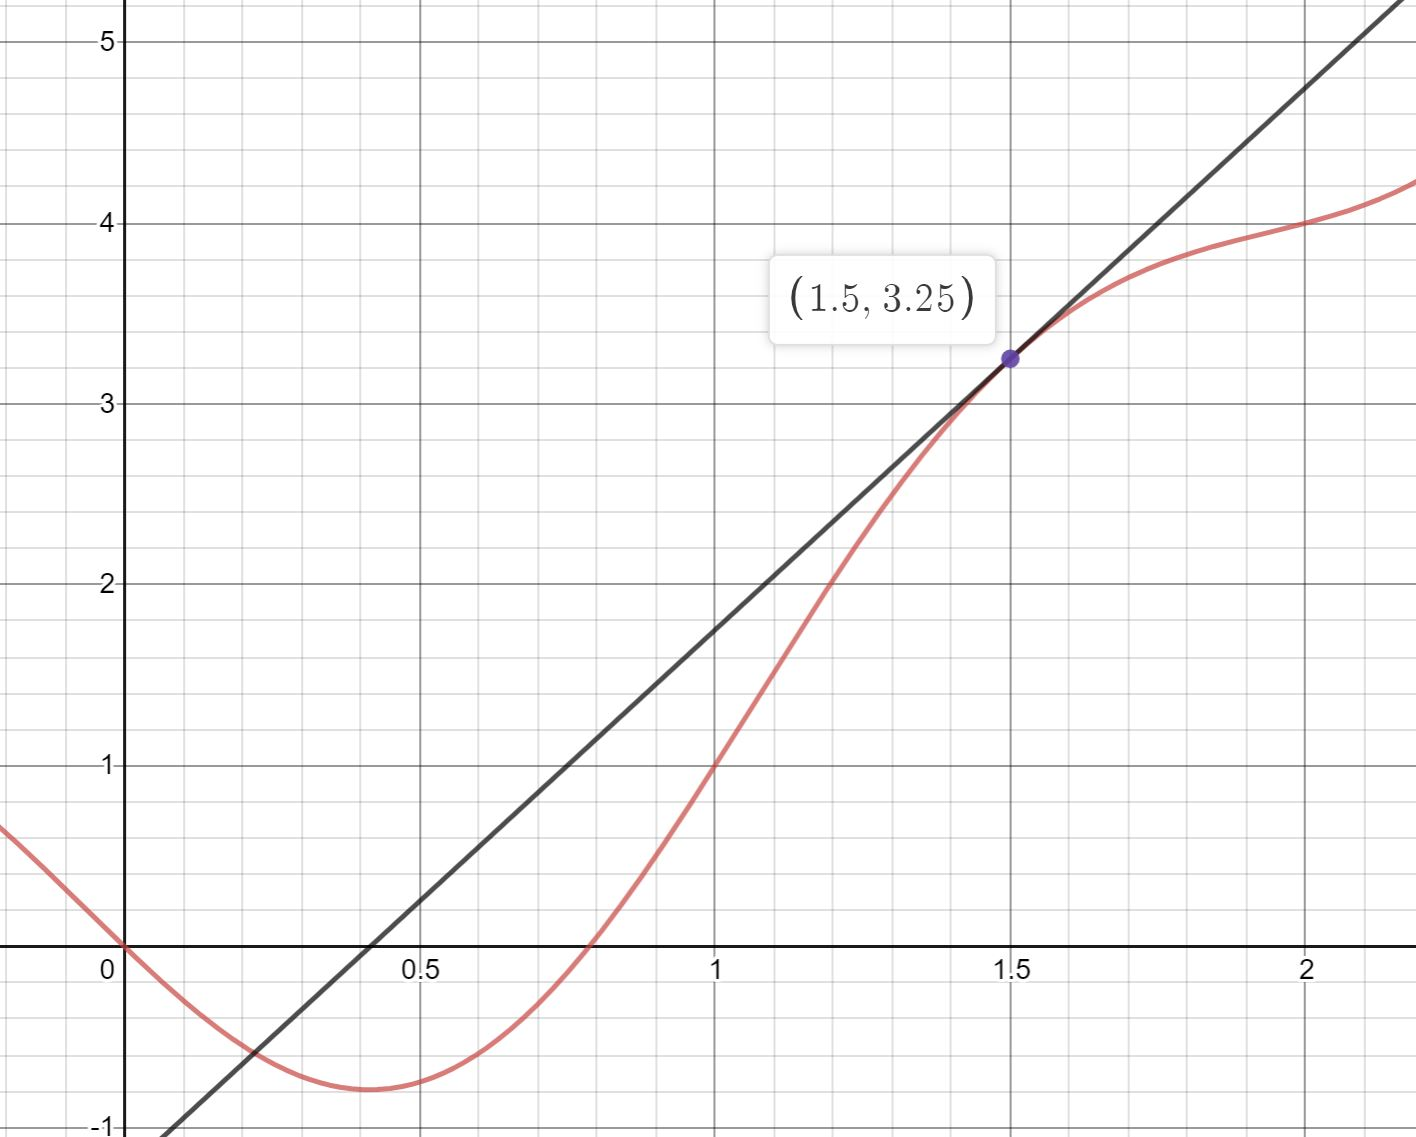
\includegraphics[height=1in]{HW6pic1.jpg}~
 
\end{image}

Use linearization to estimate $f(1.7)$.

The derivative of the function is:
$$f'(x)=\answer{2x-\pi\cos(\pi x)}$$

The slope of the tangent line at $x=1.5$ is  $\answer{3}$.

The equation of the tangent line is:
$$y=\answer{3x-1.25}$$
Enter your estimate to two decimal places:
$$f(1.7)\approx \answer{3.85}$$
 
 \end{problem}
 
 \begin{problem}\label{prob:240hom6prob3}
 Use linearization to estimate $\sqrt{10}$.

The function I will use is:
$$f(x)=\answer{\sqrt{x}}$$

The derivative of the function is:
$$f'(x)=\answer{0.5x^{-0.5}}$$

Next, I need to find the tangent line to the graph of $f$ at $x=\answer{9}$.

The slope of the tangent line is (enter exact fraction; no decimals) $\answer{\frac{1}{6}}$.

The equation of the tangent line is:
$$y=\answer{\frac{1}{6}x+\frac{3}{2}}$$
Enter exact fraction for the final answer:
$$\sqrt{10}\approx \answer{\frac{19}{6}}$$
 \end{problem}
 
  \begin{problem}\label{prob:240hom6prob4}
  The radius of a circle was measured to be 12 cm with a possible error in measurement of at most $\pm 0.1$ cm.  Use differentials to estimate the maximum possible error in the computed area of the circle.

Estimated maximum error in computed area is $\pm\answer[tolerance=0.1]{2.4\pi}$ $cm^2$.
  \end{problem}
  
   \begin{problem}\label{prob:240hom6prob5}
The table below summarizes the data collected from a remote-controlled car moving along a number line.  

\begin{center}
\begin{tabular}{|c|c|c|}
Time & Position & Velocity  \\
 \hline
 \hline
   & &\\
 2 & 4  & 3 \\
  & &\\
  \hline
   & &\\
 4 & 6 & 0.5\\
  & &\\
 \hline
  & &\\
 6 & 4 &-1 \\
  & &\\
 \hline
 \end{tabular}
\end{center}

Use this information to predict the position ($S$) of the car at the given time $t$.

$$s(2.1)\approx\answer{4.3}$$
$$s(3.9)\approx\answer{5.95}$$
$$s(6.2)\approx\answer{3.8}$$

\end{problem}

 \end{document} 